\subsection{Blended Isogeometric Discontinuous Galerkin (BIDG) Method}
\label{sec:isogeometric}

% DG
The discontinuous Galerkin method is a finite element method that excels in
aspects of its computational efficiency in the context of modern architectures,
particular in convection-dominated flows.  These allow for localization of
finite element stencils in such a way that dynamic problems lead to block
diagonal matrix systems.  The locality of the memory footprint in these
application models leads to the ability to compute solutions at high local
order and large floating point throughput \cite{Klockner20097863}.

% Iso
In traditional isogeometric analysis, computer aided design (CAD) mesh
automation tools for complex geometric domains have been developed for
triangles in two dimensions \cite{Engvall2016378} and generalized elements in
three dimensions \cite{EngvallPress}.  This allows for meshes that exactly
preserve underlying geometry in real-world designs, including both arbitrarily
smooth and discontinuous features.  In many applications, geometric
sensitivities can dominate errors \cite{Michoski2016658,Wirasaet2015597},
necessitating geometrically consistent meshes for accurate solutions at high
polynomial order.

% BIDG
The BIDG algorithm developed in \cite{Michoski2016658} merges key capabilities
offered by both isogeometric analysis and discontinuous Galerkin methods.  It
uses a piecewise rational isogeometric basis for the geometry, and a piecewise
discontinuous polynomial representation for the model, while providing an exact
(and properly conditioned) geometric transformation between the two spaces. The
BIDG method is an inherently high-order method that is amenable to
$hp$-adaptive schemes, and shows requisite super-exponential convergent
behavior.

The software package ArcSyn3sis implements the BIDG method and it is used here
for the scaling study on the KNL architecture.

\begin{figure}
\begin{center}
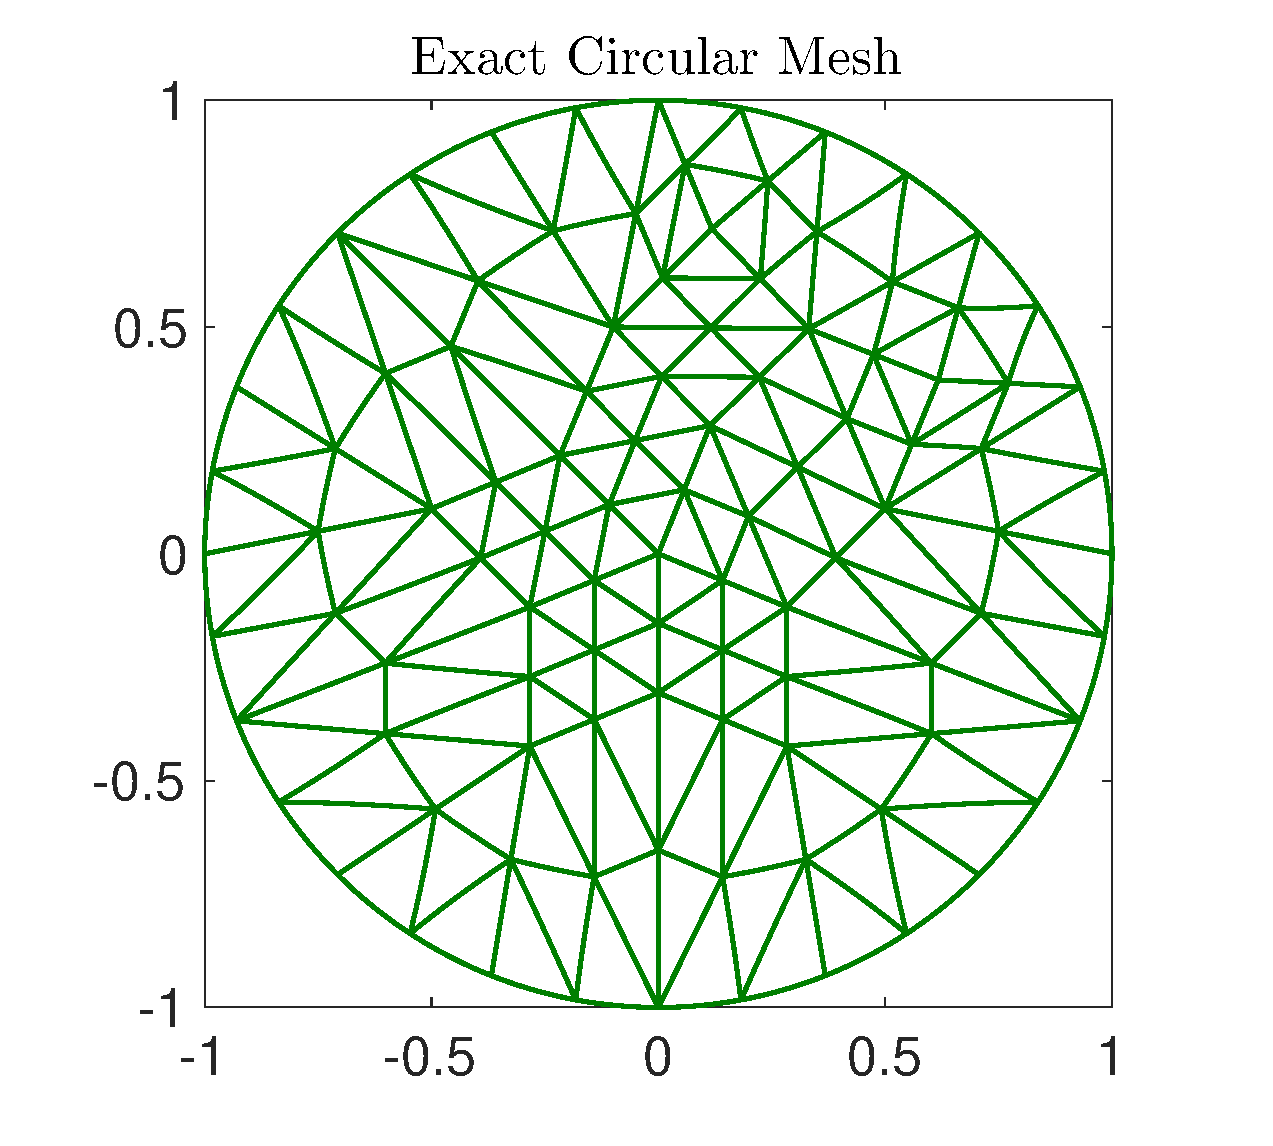
\includegraphics[width=0.8\linewidth]{./bidg_data/168_circ}
\end{center}
\vspace*{-.5cm}
\caption{Exact b\'{e}zier circular mesh used in the scaling study.}
\label{fig:168_circ}
\end{figure}

For our scaling test here we solve the first-order acoustic wave equation:
\begin{equation}
  \label{awe}
  \frac{\partial p}{\partial t} + \nabla\cdot \boldsymbol{u} = 0, \quad
  \frac{\partial\boldsymbol{u}}{\partial t} + \nabla p = 0,
\end{equation}
where $\boldsymbol{u}=(u_x,u_y)$ is the velocity, and $p$ the pressure.

Such a system is discretized by solving the semidiscrete block diagonal system
\[
  \left( v, \frac{ \partial A}{\partial t} \right)_{\Omega_{i}} =
  V_{\Omega_{i}}+S_{\partial\Omega_{i}}
\]

for $A = (p,\boldsymbol{u})$, $V_{\Omega_{i}}$ a volume intergral that has only
elementwise dependencies, and $S_{\partial\Omega_{i}}$ a surface integral that
depends on inter-element communication through classical upwinding
\cite{Michoski2014898}.  The volume integral can be written in three nested
loops; the outer looping over elements, and two inner loops over degrees of
freedom in the DG basis.  The surface intergral similarly loops over elements,
but then due to an additional interpolation step from the isogeometric
transformation, extends one of these nested loops over the quadrature degrees
of freedom for curved edges.  The resulting linear system that is solved,
$Fx = b$ admits an attractive block-diagonal structure,
\begin{equation}
  F = \begin{pmatrix}
    F_1 & 0 & \cdots & 0 \\
    0 & F_2 & \cdots & 0 \\
    \vdots & & \ddots & \vdots \\
    0 & 0 & \cdots & F_n \\
  \end{pmatrix},
\end{equation}
and this highly motivates the use of a many-core architecture for execution.

\begin{figure}
\begin{center}
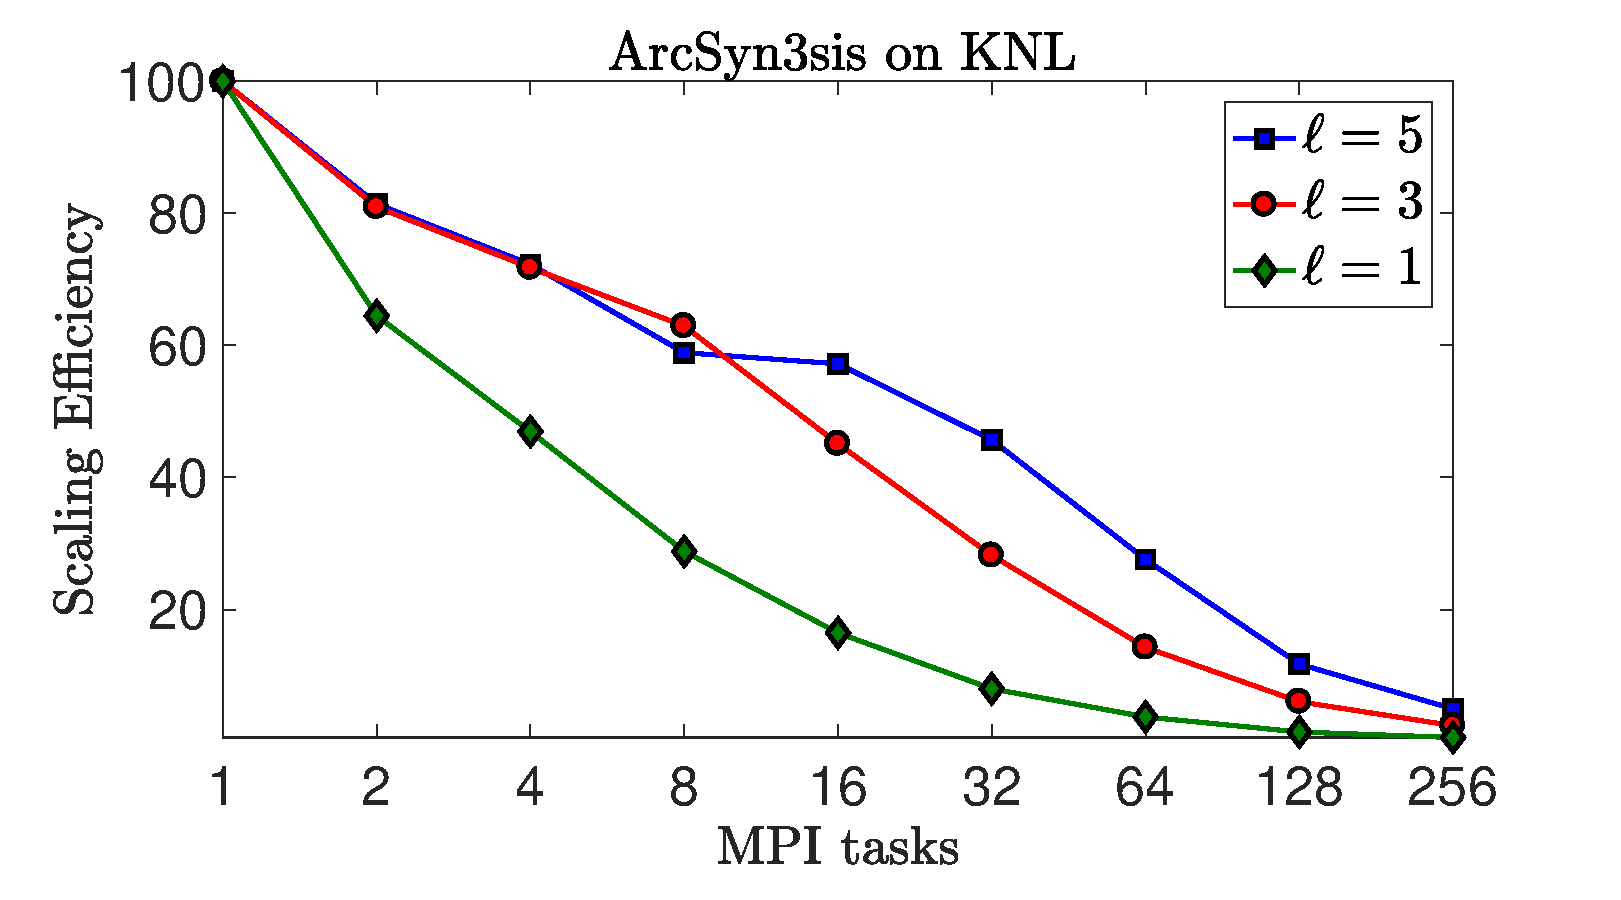
\includegraphics[width=0.99\linewidth]{./bidg_data/2nd_try/scaling}
\end{center}
\vspace*{-.5cm}
\caption{Strong scaling of the ArcSyn3sis BIDG kernel on KNL nodes run on
isogeometric 168 element mesh, and shown at different polynomial order $\ell$.}
\label{fig:bidg_scaling}
\end{figure}

The implementation on isogeometric meshes utilizes the Open Concurrent Compute
Abstraction (OCCA) library \cite{MedinaPress}.  The OCCA library abstracts
multiple threading back-ends OpenMP, OpenCL, and CUDA using a C preprocessor
macros.

% The OCCA kernel implements macro-based just-in-time code
% generation so that the platform target can be identified at runtime.  Threaded
% barriers are also set in the application kernel to allow for thread-based
% granularity, giving more flexibility during code optimization.  The
% implementation of the ArcSyn3sis kernel using OCCA allows for aliasing, of e.g.
% flattened cache-line boundary aligned arrays, such that data structures can be
% called more intuitively (e.g.  a 4-tensor can be called as a four array,
% instead of indexed as a flattened contiguous one array).

The results of the basic scaling study are shown in
Fig.~\ref{fig:bidg_scaling}, where the strong scaling efficiency $e_{n}$ for
$n$ MPI tasks is defined as $e_{n}= [t_{1}/(nt_{n})]\times 100\%$, setting the time to
completion as $t_n$. These preliminary results seem to indicate improved scaling as a function of polynomial order $\ell$, which is consistent with the theoretical
behavior of the algorithmic intensity of DG algorithms.  However, this is
clearly not enough evidence to be certain that such scaling is being observed.
In particular, on this mesh we see an efficiency saturation above $\ell>5$.
Moreover, since the mesh itself has only 168 elements, the number of threads
eventually exceeds the number of elements, making for some intriguing questions
regarding the observed behavior.  In order to fully understand the observed behavior and
optimize the code appropriately, a more extensive study is required, including
%a streams
%
%NM-- why streams? Streams is just a memory bandwidth benchmark. If this is
%     expected to be the bottleneck, I would directly address that in the text.
%CM -- Nick, sorry, I don't understand your point.  I don't know what the bottleneck is because I have not done comprehensive tests, so I can't rule out a bottleneck until I run the tests.  All I can do is guess.  Memory bandwidth may very well be causing a problem, and the vector kernels should be tested.  On the other hand, I think the roofline model would cover this too, so we can delete it if you prefer?
%benchmark \cite{McCalpin1995} and
a roofline performance test
\cite{Williams:2009:RIV:1498765.1498785}.

%
% NM --- feel free to disregard anything I recommend here
%
 %yar\todo{Discuss, broadly, what class of problems this resides in and why humanity works on it}

%% yar2\todo{some basic intro to the linear algebra you are doing}

%% yar3\todo{any nuances of porting to MIC?}

%% yar4\todo{discussion of scalability observed}

%Finally, some discussion is needed: is DG ameniable to MICs? Vs typical CPUs? I
%naively guess so, since you can essentially vectorize several of the
%activities.
